\documentclass[12pt]{article}
\usepackage[margin=2.5cm]{geometry}
\usepackage[version=4]{mhchem}
\usepackage{graphicx}
\usepackage{subcaption}
\usepackage{placeins}
\usepackage{minted}
\usepackage{wrapfig}
\usepackage{fancyhdr}
\usepackage{lastpage}
\usepackage{hyperref}

\setlength\parindent{0pt}

\pagestyle{fancy}
\fancyhf{}
\renewcommand{\headrulewidth}{0pt}
\cfoot{\thepage \ / \pageref{LastPage}}

\begin{document}

\begin{titlepage}
    \begin{center}
        \vspace*{1cm}
        \Huge
        \textbf{NMR spectroscopy internship}
        
        \vspace{0.5cm}
        \LARGE
        Supervisor: RAYA Jesus
        
        Research team of Prof. Bechinger
        
        \vspace{1.5cm}
        \textbf{Louis-Hendrik Barboutie}
        
        \vfill
        

        
\includegraphics[width=0.4\textwidth]{logo_institut.png}
        
        \Large
        28th August to 30th September 2022
    \end{center}
\end{titlepage}

\tableofcontents
\newpage
\listoffigures
\listoftables
\newpage

\section{Introduction}

\subsection{The institute and research team}

\subsection{The HyCGreen Project}

\section{A very brief introduction to NMR spectroscopy}

This section is in no way a complete explanation of NMR spectroscopy and many details are glossed over. Refer to J. Keeler "Understanding NMR spectroscopy" for more in-depth and rigorous description.

\subsection{Nuclear Spin and Magnetization}
\begin{wrapfigure}{r}{0.45\textwidth}
    \centering
    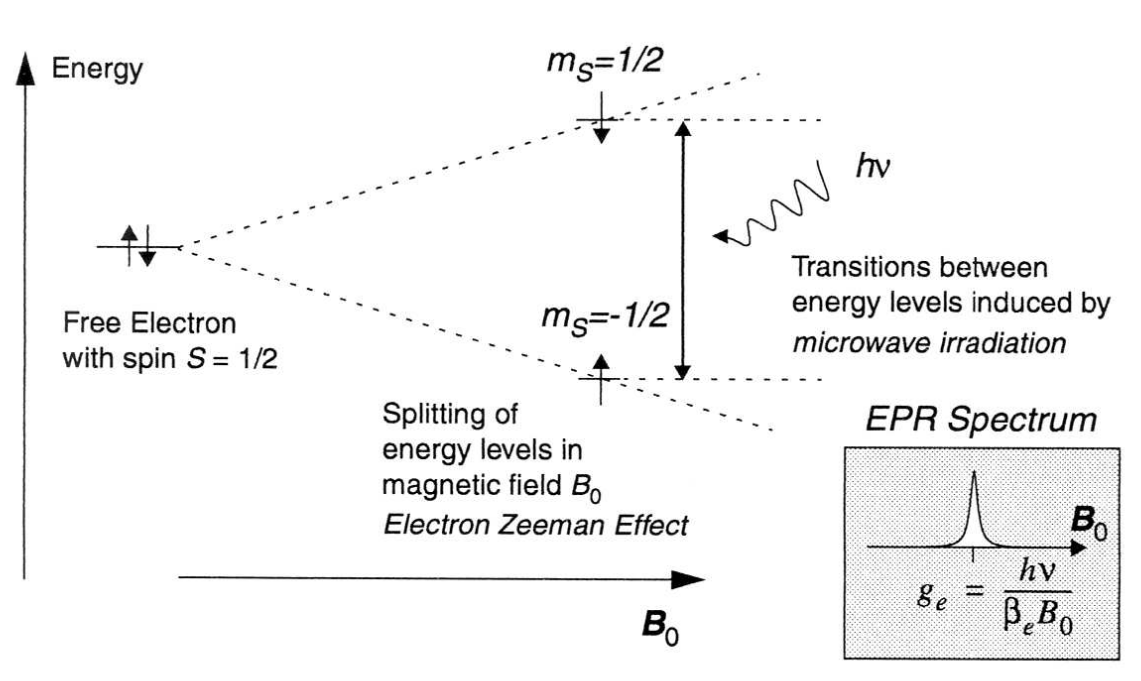
\includegraphics[width=0.45\textwidth]{ZeemanEffect.png}
    \caption{Zeeman Effect}
\end{wrapfigure}
Atomic nuclei have an intrinsic property, like mass or electric charge, called spin, which is the foundation of NMR spectroscopy. For our considerations, the spin can be thought of as a magnet, as it interacts with magnetic fields. A particle with spin quantum number $s$ can be in the spin state $m_s = s$, $m_s = s-1$, $m_s = s-2$, ..., $m_s = -s$. This means a particle with spin $s=\frac{1}{2}$ has two possible spin states: $m_s = \frac{1}{2}$ and $m_s = -\frac{1}{2}$. These states are degenerate, ie. it is not possible to distinguish the two in terms of energy. This degeneracy can be lifted by applying a strong external magnetic field, with which the spins will interact: they align either parallel or antiparallel. With this alignment comes a small energy difference which differentiates the two spin states; this is known as the Zeeman-Effect. 

NMR spectroscopy works best with spin $s=\frac{1}{2}$ nuclei. The distribution of the populations of spin-up and spin-down nuclei is governed by a Boltzmann distribution. Transitions from one state to the other are possible when the nuclei are hit by electromagnetic radiation of frequency $\nu$ that fulfill the condition: $\Delta E = h \nu$, where $\Delta E$ is the energy difference between the spin-up and spin-down state. When these transitions happen continuously, the frequency is said to be the resonance frequency. While quantum mechanics tell us the individual spin orientation cannot be precisely measured, there is in fact a net magnetization arising from a sample: the addition of the spin lead to a macroscopic, observable quantity. Because of the population distribution, it is aligned parallel or antiparallel to the external field.

If a magnet is placed in an external field, and is not aligned to it, it will feel a torque and follow a precessing motion. it will rotate around the axis of the external field similarly to how a gyroscope behaves. The frequency of precession is called the Larmor frequency and is actually independent of the polar angle between the magnetization vector and the external field. It also follows a nutation motion, which brings it back in alignment with the external field. This phenomenon is also happening with the spin induced magnetization of a sample.

\subsection{Rotational frame of reference}

\subsection{Interactions}

\subsubsection{Chemical shift}

Every atom and molecule in a sample has its own electron cloud. Electrons also have a spin and produce their own magnetic field, that shields the nuclei from the external field B$_0$. This means that the nuclei will see an effective field, which is reduced due to the shielding. The Larmor frequency though depends on the field, and therefore a shift is observed. The chemical shift is also influenced by the orientation of the molecule or atom in the external field

\subsubsection{Dipolar coupling}

Dipolar coupling occurs as two spins interact with each other. Each spin produces a magnetic field, which can be sensed by other spins and lead to spin flipping. This phenomenon also has a repercussion on the final spectrum: instead of having a clean peak, there is a double peak called pake doublet.

\subsection{The NMR spectroscope}

The NMR spectroscope is in principle a simple construction. An external field is produced by a superconducting magnet plunged in liquid helium, and surrounded by a liquid nitrogen shell. The real magic happens inside the bore containing the sample. The sample is inside a coil, which works both as Radio Frequency (RF) emitter and measurement unit. A moving magnet will induce electric currents, and the same is happening with the spin induced magnetization, and can thus be detected by the emitter. A RLC circuit allows for precise control over the impedance of the whole construction. NMR spectroscopy isn't very sensitive and it is therefore important to acquire a maximum of signal, and thus the circuit needs to be 'tuned' and 'matched' so that the resonance frequency corresponds to the frequency with the minimum absorbed voltage.

The emitter coil allows to tilt the net magnetization by emitting short pulses at the Larmor frequency and enables the recording of the Free Induction Decay (FID), which is the the signal observed until the magnetization stabilizes parallel to the field again. Using mathematics and wave properties, it is possible to recover both the real and imaginary parts of the signal. Finally a Fourier Transform is applied to obtain a spectrum.

The probe has three simultaneous channels for acquisition. In essence, each channel makes it possible to pulse at the frequency of different nuclei, via the same coil. Similarly to how an antenna can emit and receive multiple frequencies at the same time, the coil creates multiple B$_1$ fields, for each channel. Since this secondary field has an insignificant strength against the external field, unless it is on resonance, the multiple fields won't have an interference effect.

Inside samples molecules interact and such interactions can be undesirable but these can be 'removed' by Magic Angle Spinning (MAS). This technique also comes in handy for solid spectroscopy, as solids often are very heterogeneous and the spinning averages out interaction, similarly to the brownian motion in liquids. For MAS to work, the sample needs to be tilted to approximately 54.7$^{\circ}$, and spun at rates in the kHz range (usually 2-130 kHZ).

\subsection{NMR aquisition techniques: Pulse programs and acquisition sequences}

Pulse programs play an important role in NMR: they can improve the signal to noise ratio and thus make better spectra. A very famous one is the Spin Echo sequence, also known as Hahn echo.

\subsubsection{Hahn echo}

Because of inhomogeneities in the external field, the actual precession speed of the individual spins is not the same everywhere: Some preceed faster and some slower, leading to a dephasing. The Hahn echo sequence counteracts this by periodically applying 180° pulses. This leads to the faster precessing spins to catch up on the slower precessing ones and to refocus the magnetization. The Hahn echo sequence greatly improves the signal to noise ratio. Follow the link for an animation of a single echo: \href{http://xrayphysics.com/se\_3d.gif}{\textit{click me}}   

\subsubsection{Cross polarization}

Sometimes, the signal we obtain from a nucleus isn't very strong, but there is a remedy for that: Cross Polarization (CP). In essence, it is a transfer of magnetization via dipolar coupling from a more abundant nucleus to the one we want to observe. CP only works in static solid NMR as during MAS NMR dipolar couplings are averaged.

\subsubsection{Spin Exchange at Magic Angle (SEMA)}

Proton-proton interactions are problematic if there are other heteronuclear interactions we want to observe, eg. proton-nitrogen or proton-carbon. Luckily, there is a way to "spin lock" the protons and stop this interaction from happening. This is achieved by setting an RF frequency on the proton channel, such that in the rotational frame of reference the effective field of the nuclei is oriented at the magic angle. The technique is called SEMA, and is used for static solid NMR. 

\section{Experimental results and discussion}

\subsection{Theory}

The used experimental process is Magic Angle Spinning Nuclear Magnetic Resonance spectroscopy (MAS NMR). It is based on the property of certain nuclei to have a non-zero total spin. The technique is very effective when observing $^1$H, $^{13}$C or N.

A very powerful magnet creates a strong magnetic field, in which the spins from the individual nuclei orient themselves. They point either parallel or antiparallel to the applied field. Because the proportions of both populations isn't the same, a net magnetization can be observed. The magnetization is a macroscopic observable.

While great care is being taken in regulating the temperature of the sample, some effects cannot be avoided. During the spinning process, the air used to create the bearing and to induce the rotation is not thermally controlled. There is also friction-induced heating due to the rapid spinning. The heating of the sample is usually not homogeneous, there is a temperature gradient inside, as there are temperature differences in different places. The temperature has a noticeable effect on the spectrum: it increases the chemical shift. With a very heavy nucleus, e.g. Lead ($^{207}$Pb), this increase can be detected with high sensitivity. In order to get rid of the gradient, the sample is given some time to accommodate to a given temperature

\subsection{Calibration of the temperature}

\subsubsection{Preliminary theory}

Since the thermocouple giving us a reading of the temperature inside the probe is placed outside of the capsule containing the sample, the value we are getting is true only to some degree. In addition, the thermocouple needs calibration, ie. the temperature reading might be off by a few kelvin. It is not possible to put a thermocouple in direct contact with the sample, therefore we need another way of determination of the temperature.

We can remedy to that by performing static spectra. If we use the chemical shift difference between $\delta_{peak}$ and $\delta_{iso}$, we get a value independent of the (eventually false) calibration. Using the equations provided by Beckmann and Dybowski, the true temperature $\theta_{abs}$ can determined:

The equations given are
\[
\begin{cases}
    \delta_{peak}(\theta) = (0,666 \pm 0,003 \ \text{ppm}\cdot\text{K}^{-1}) \cdot \theta + (-3670,6 \pm 1,0 \ ppm) \\
    \delta_{iso}(\theta) = (0,758 \pm 0,002 \ \text{ppm}\cdot\text{K}^{-1}) \cdot \theta + (-3713,9 \pm 1,0 \ ppm) 
\end{cases}
\]
\[
\theta_{abs} = \frac{(43,3 \pm 2,0 \ \text{ppm} ) + (\delta_{iso} - \delta_{peak})}{(0,092 \pm 0,005 \ \text{ppm} \cdot \text{K}^{-1})}
\] \medskip

If the thermocouple gives a different value from $\theta_{abs}$, it can be adjusted accordingly. The spectrum can finally be calibrated on the peak or chemical shift anisotropy using $\delta_{peak}(\theta_{abs})$ or $\delta_{iso}(\theta_{abs})$

From this point on, the temperature for the static sample can be used as a reference for the change in temperature when the sample is spinning. Not only is it possible to know the temperature of the sample, but also to observe the way the temperature increases. If the temperature is known, it can also be used to predict the induced chemical shift.

\subsubsection{Application}

Static spectra are taken for three different temperatures: 255 K, 273 K and 295 K. Then for each spectrum, $\delta_{iso} - \delta_{peak}$ is calculated. With three points on hand, the thermocouple can then be calibrated. Hahn spin-echo sequences are used to maximize the signal to noise ratio, and then the spectra are fitted with ideal curves. Below are the spectra obtained for each temperature.

\begin{figure}[!ht]
    \centering
    \begin{subfigure}[b]{0.3\textwidth}
        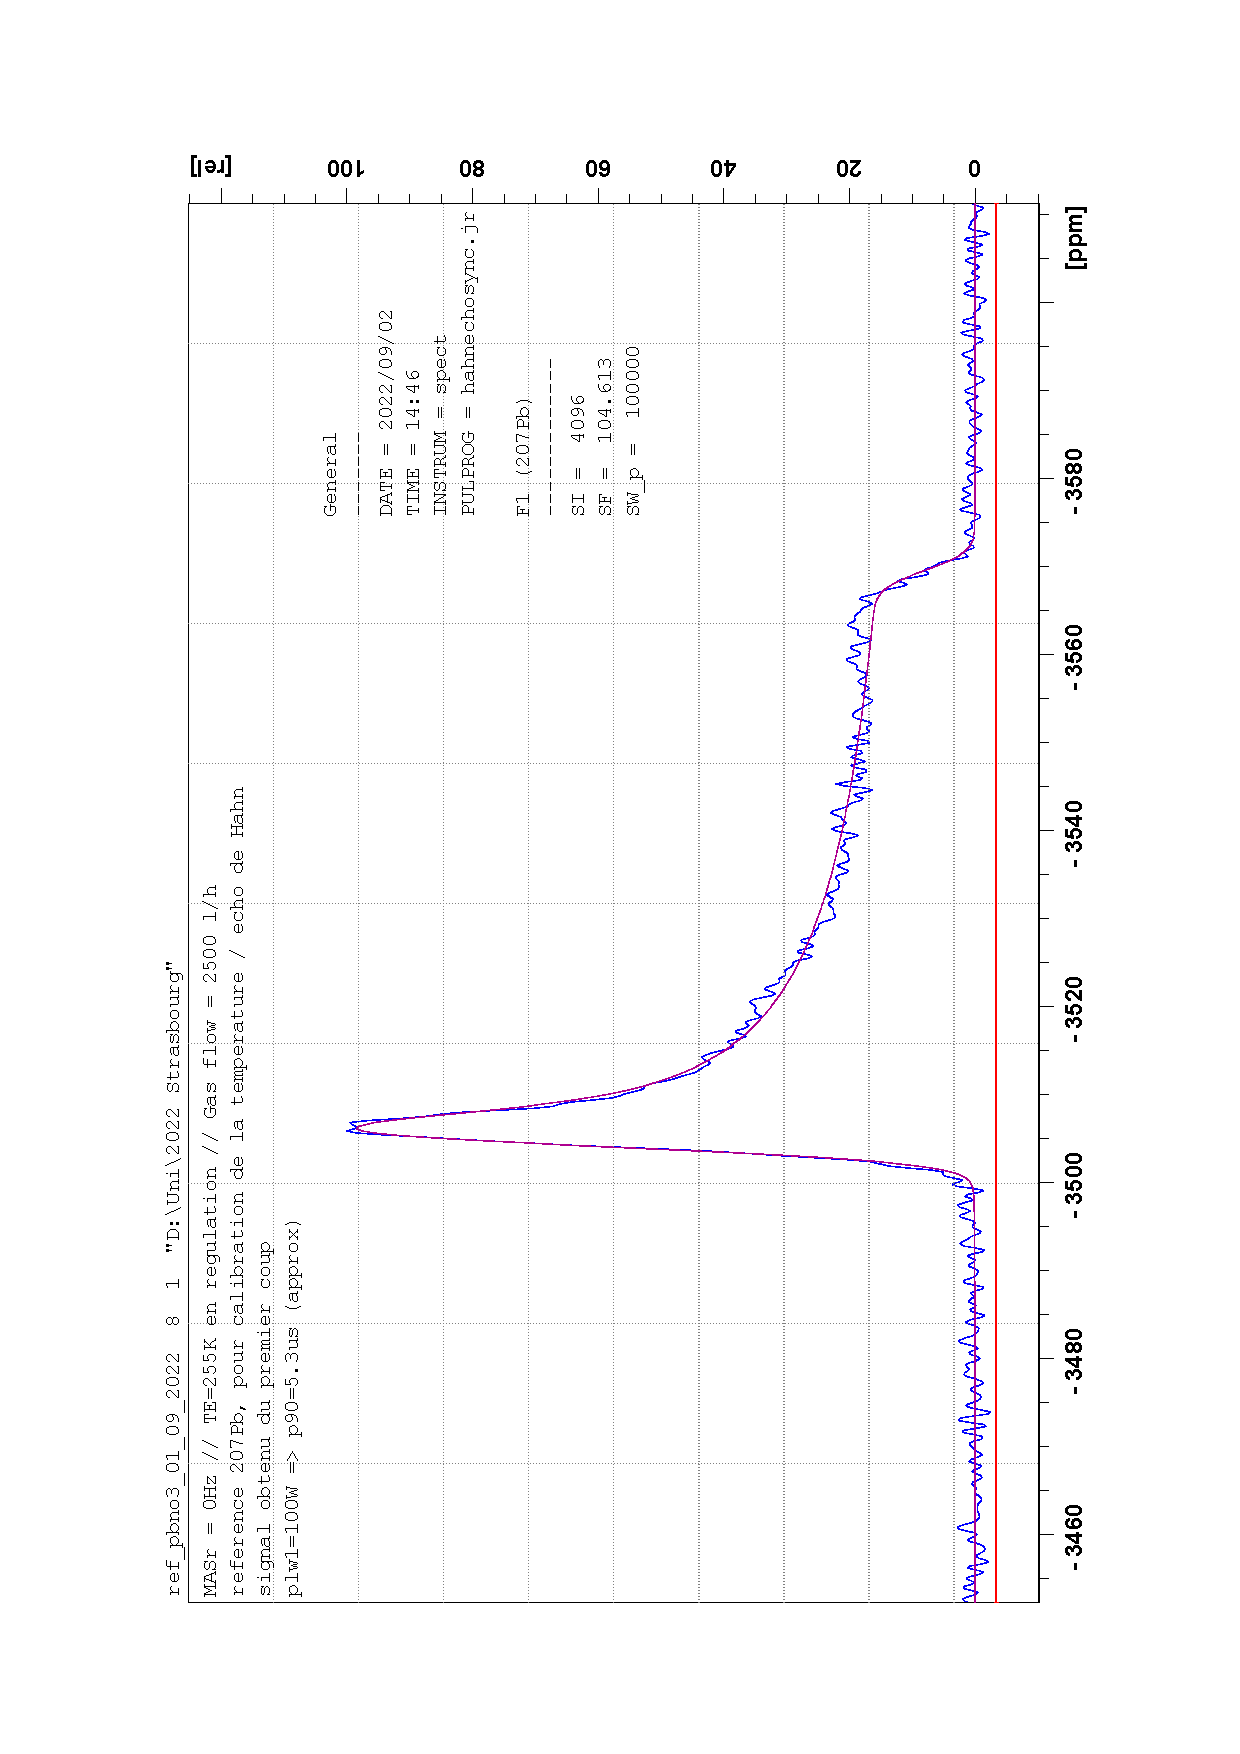
\includegraphics[width=0.8\textwidth,angle=-90]{207Pb/207Pb_255K.pdf}
    \end{subfigure}
    \begin{subfigure}[b]{0.3\textwidth}
        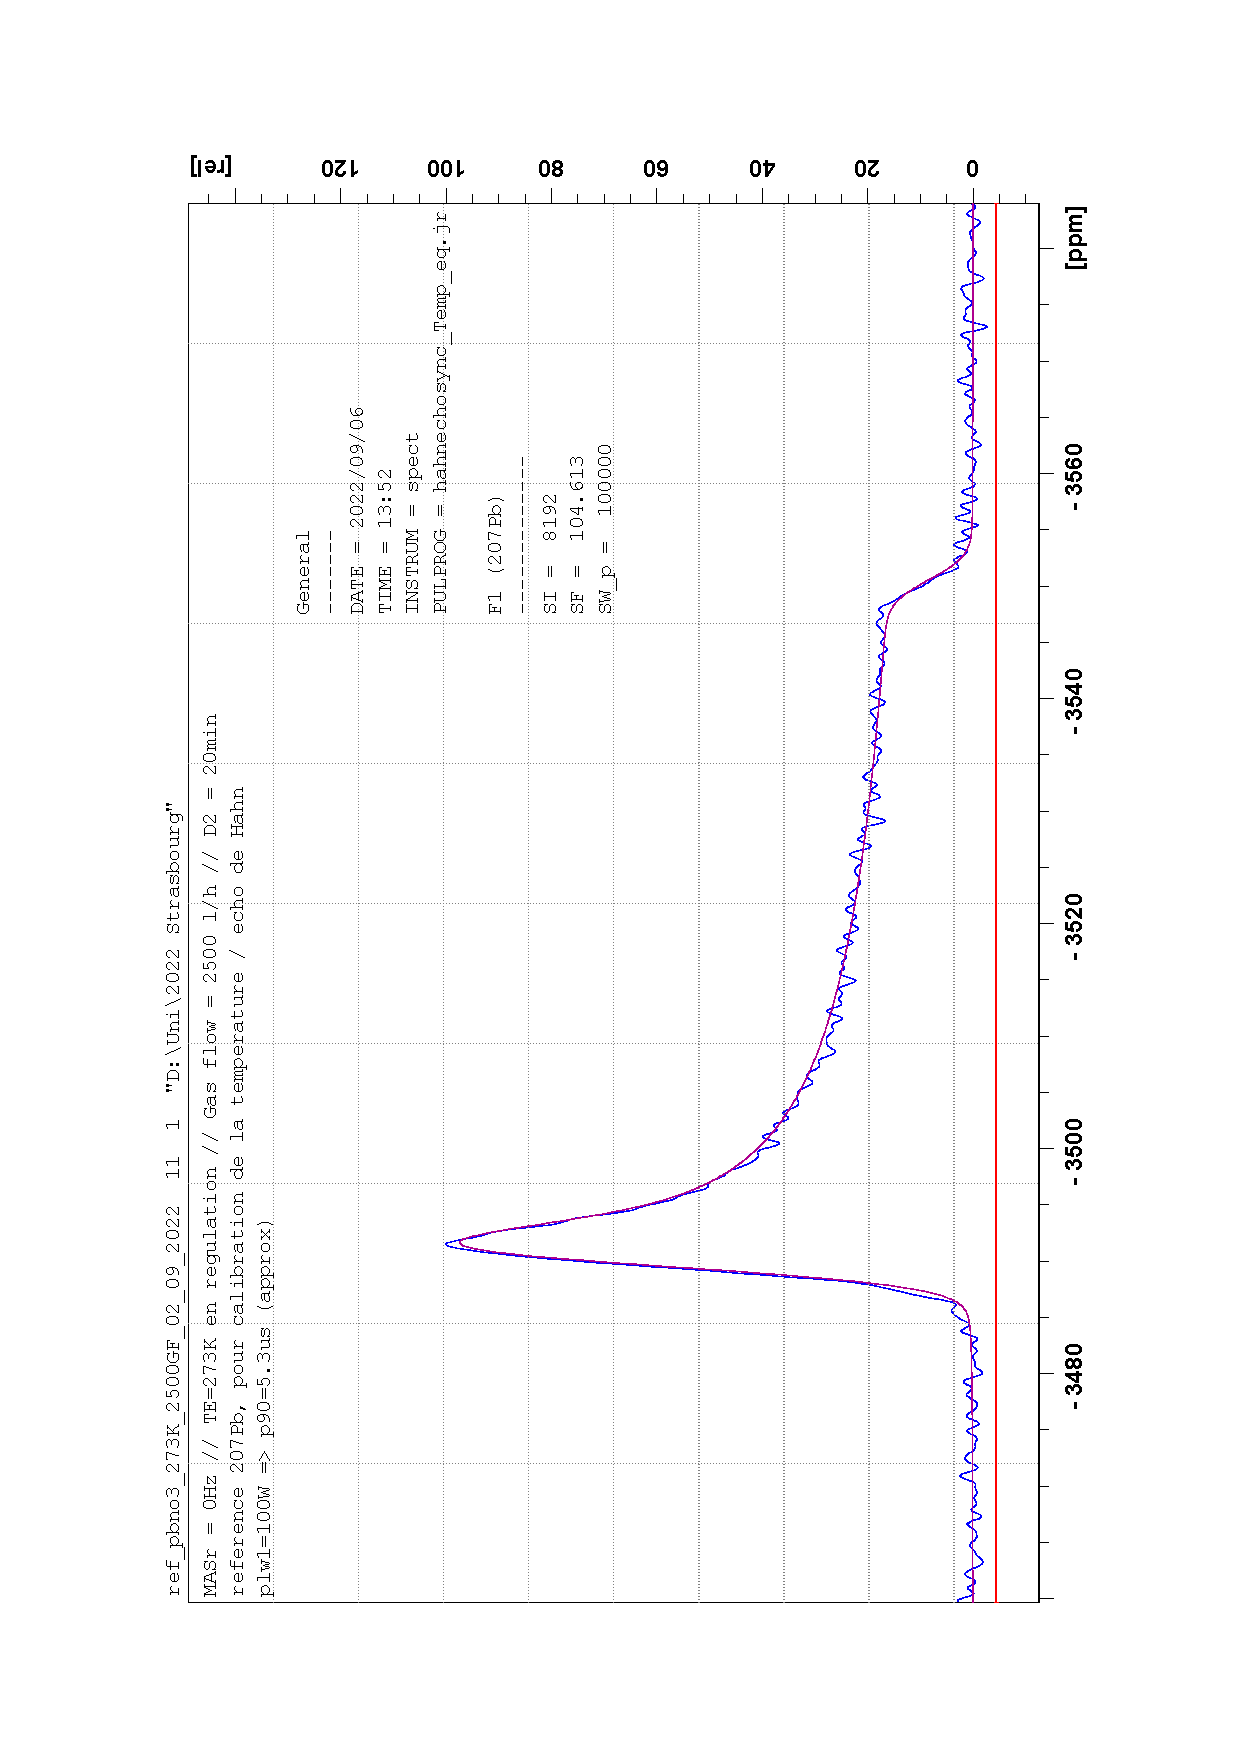
\includegraphics[width=0.8\textwidth,angle=-90]{207Pb/207Pb_273K.pdf}
    \end{subfigure}
    \begin{subfigure}[b]{0.3\textwidth}
        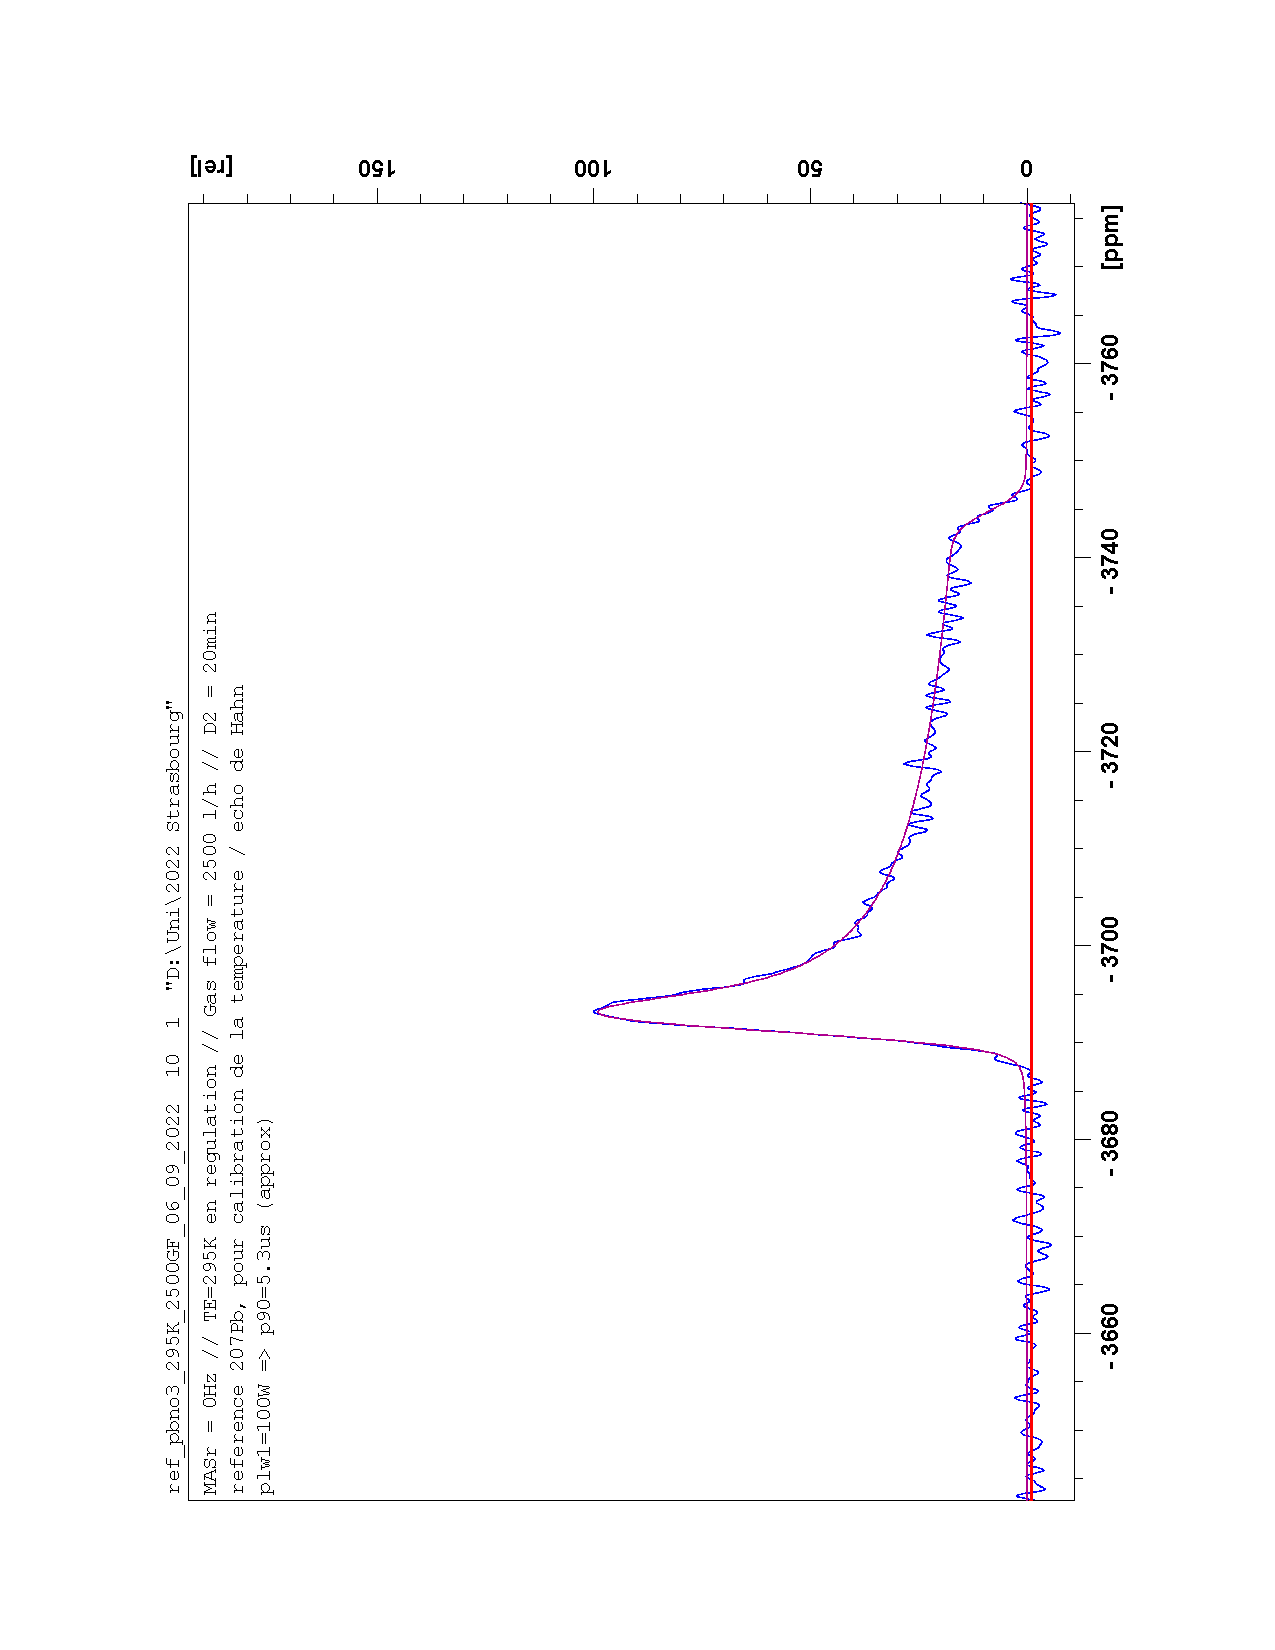
\includegraphics[width=0.8\textwidth,angle=-90]{207Pb/207Pb_295K.pdf}
    \end{subfigure}
    \caption{Caption}
    \label{fig:my_label}
\end{figure}

For each spectrum we can find the $\delta_{iso}$ and the $\delta_{peak}$: $\delta_{peak}$ is measured in the position of highest intensity, and $\delta_{iso}$ is given by the chemical shift of the half-integral of the ideal fit curve. From the spectra above we can see that $\delta_{peak} < \delta_{iso}$.

There is however, with this method, a big issue: the uncertainty on the calculated true temperature is very high. It is due to a very generous error given on the values given by Beckmann and Dybowski. From our data, the error should be a tenth of those given.

\subsection{Static spectra with variable temperature}

Since we have a high error on our measurements, due to the generous estimate given on the equations, we still want to observe the behaviour of the spectra when we modify the temperature. For this we used the newly implemented AU-MULTI-VT-STATIC script to automate the data acquisition. With a step of 10 K, spectra were acquired for temperatures from 295 K to 255 K, and then from 260 K to 290 K, again with a step of 10 K. Just before acquisition, the sample is spun up to 5000 Hz for 300 s, and then given a minute before the spectrum is getting saved.

\begin{figure}[!ht]
    \centering
    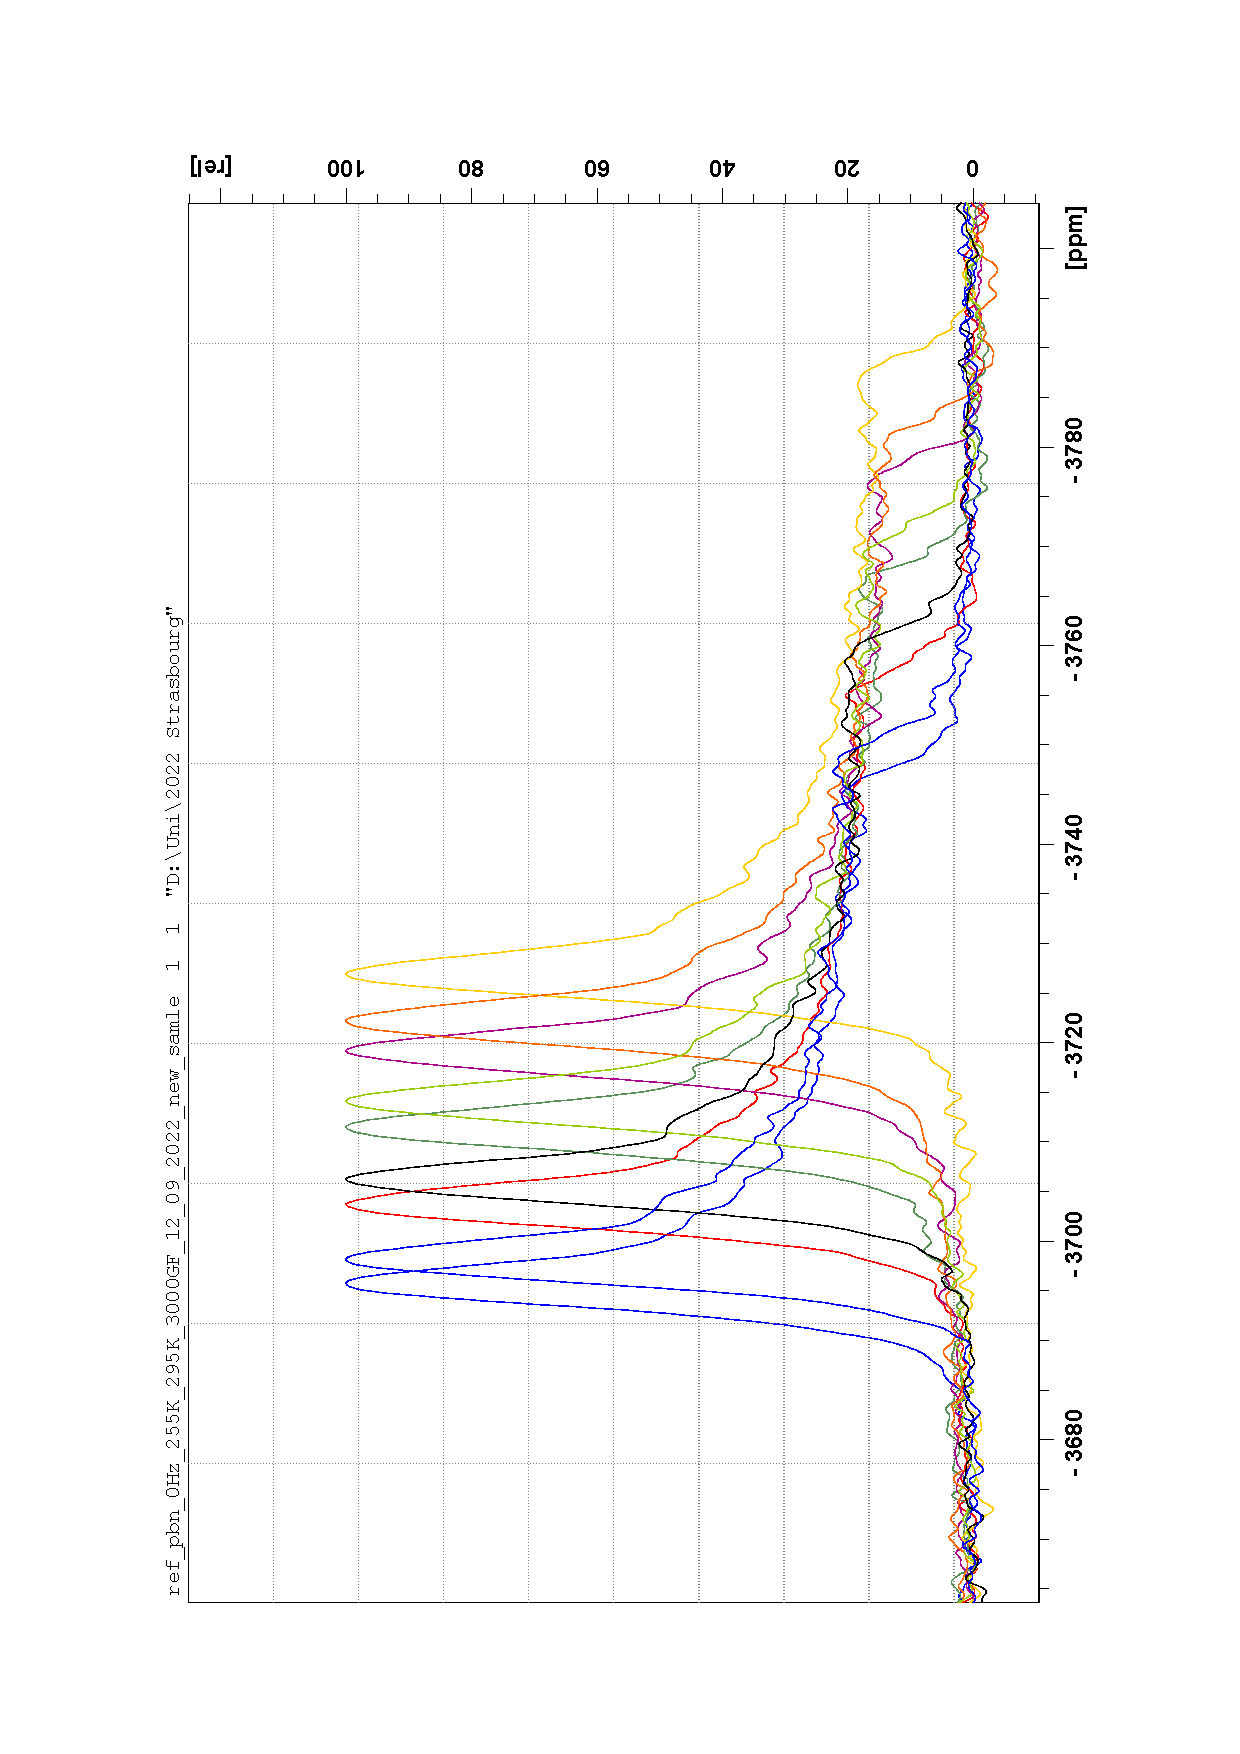
\includegraphics[width=0.7\textwidth,angle=-90]{207Pb/Static_VT_Linera_Multi_Spectra.pdf}
    \caption{Spectra obtained by the static-vt experiment}
    \label{fig:Static_VT_Linera_Multi_Spectra}
\end{figure}
\FloatBarrier

The chemical shift scales linearly with the temperature, however the slope changed from the series where temperatures were falling (black dots, blue fit), to the series where temperatures were rising (red dots, green fit). This discrepancy may indicate an insufficient thermal equilibration delay.

\begin{figure}[!ht]
    \centering
    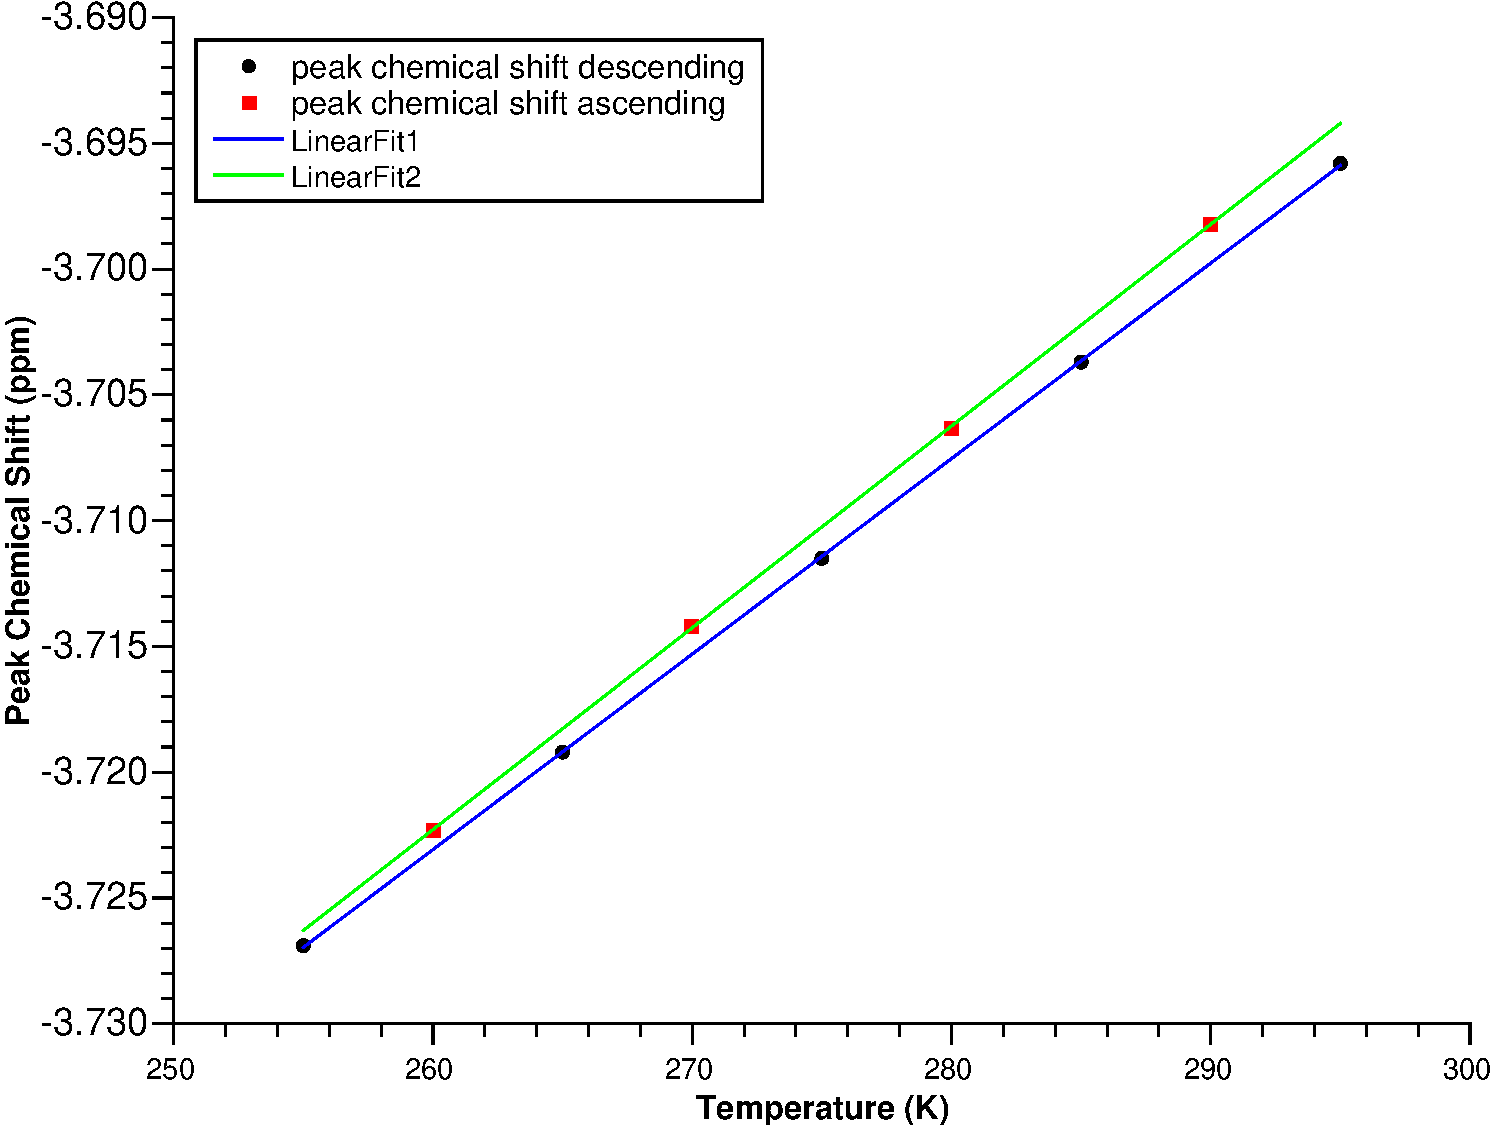
\includegraphics[width=0.7\textwidth]{207Pb/Static_VT_Linear.pdf}
    \caption{Peak Chemical Shift as a function of the Temperature in the static case}
    \label{fig:Static_VT_Linear}
\end{figure}

While the difference between the slopes seems minimal, it represents an important difference in chemical shift, and thus in the accuracy the measurement. Note that the spectra obtained in this region were obtained using a different lead sample. We were unable to get rid of the dipolar couplings to get a nice, tensor-shaped peak. After ejecting it and letting it rest outside of the magnetic field over night 'reset' the sample, and we were able to acquire regular spectra again.

\subsection{Study of the influence of rotation on the temperature}

With the previously described calibration procedure, it is now possible to study the impact of the spinners rotation on its temperature. The idea is to set a coolant temperature and then observe the chemical shift of the spectrum. The same lead nitrate filled spinner as for the calibration process is used for the study. For a given temperature, we can first record a static spectrum and us it as a reference point as zero chemical shift.

\subsubsection{Thermal equilibration time}

The cooling or heating of the spinner to a set temperature is not instantaneous, and it requires a certain delay until a measurement can be done. Else the data would still be influenced by whatever the previous temperature was set. In order to determine how much time is needed to acclimatize the sample, we perform the same experiment with various equilibration times. 

The temperature is set to 255 K, at a gas flow of 2500 L/h and in three acquisitions the sample is given 40, 60 and 80 minutes at a given speed until a measurement is done. Below is a comparison of the results:

\begin{figure}[!ht]
    \centering
    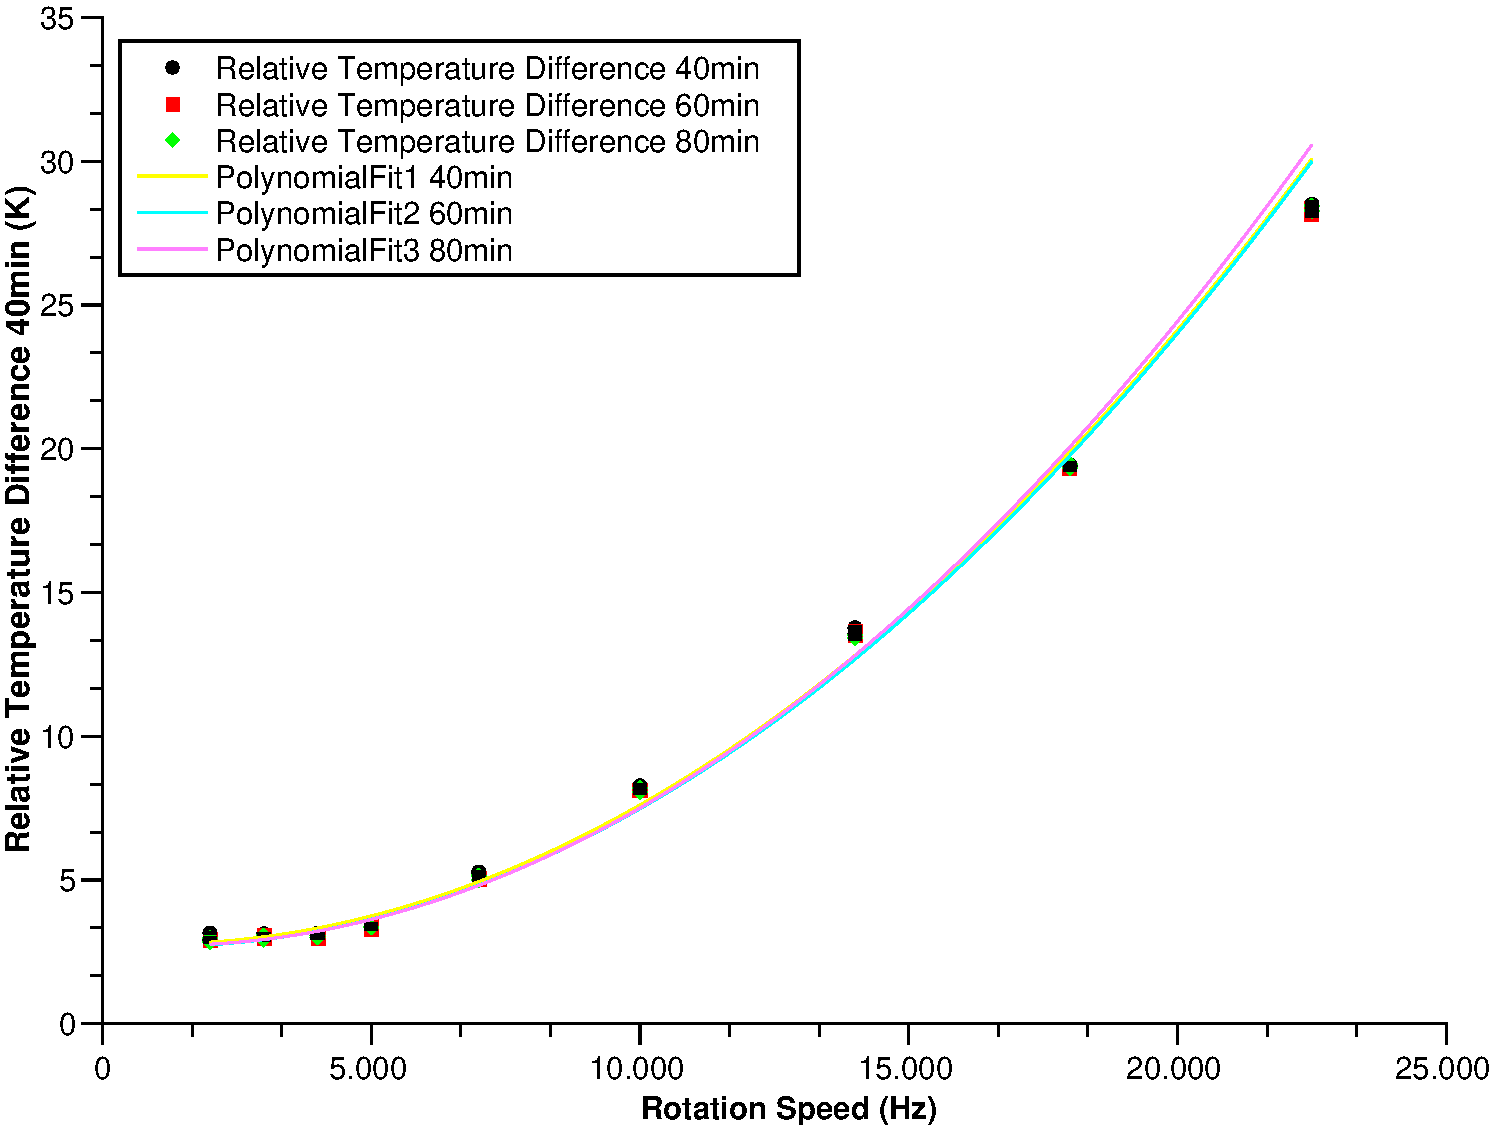
\includegraphics[width=0.7\textwidth]{207Pb/207Pb_255K_Comparison_40_60_80.pdf}
    \caption{Comparison of the relative temperature difference as a function of mas rotation speed for various thermal equilibration delays}
    \label{fig:207Pb_255K_Comparison_40_60_80}
\end{figure}
\FloatBarrier

There is very little difference between the data points, confirming that 40 min is largely enough time to let the sample acclimatize itself. We later found out, that a 20 min delay is already sufficient. The polynomial fits make the quadratic relationship between angular frequency and the temperature difference apparent.

To get a better idea of what is happening, we repeated the experiment with more data points, going in steps of 1250 Hz, and covering a range of 2500 to 22500 Hz. The temperature difference is measured for a coolant flow of 3000 L/h at 250 K. The results are in displayed in the following graph:

\begin{figure}[!ht]
    \centering
    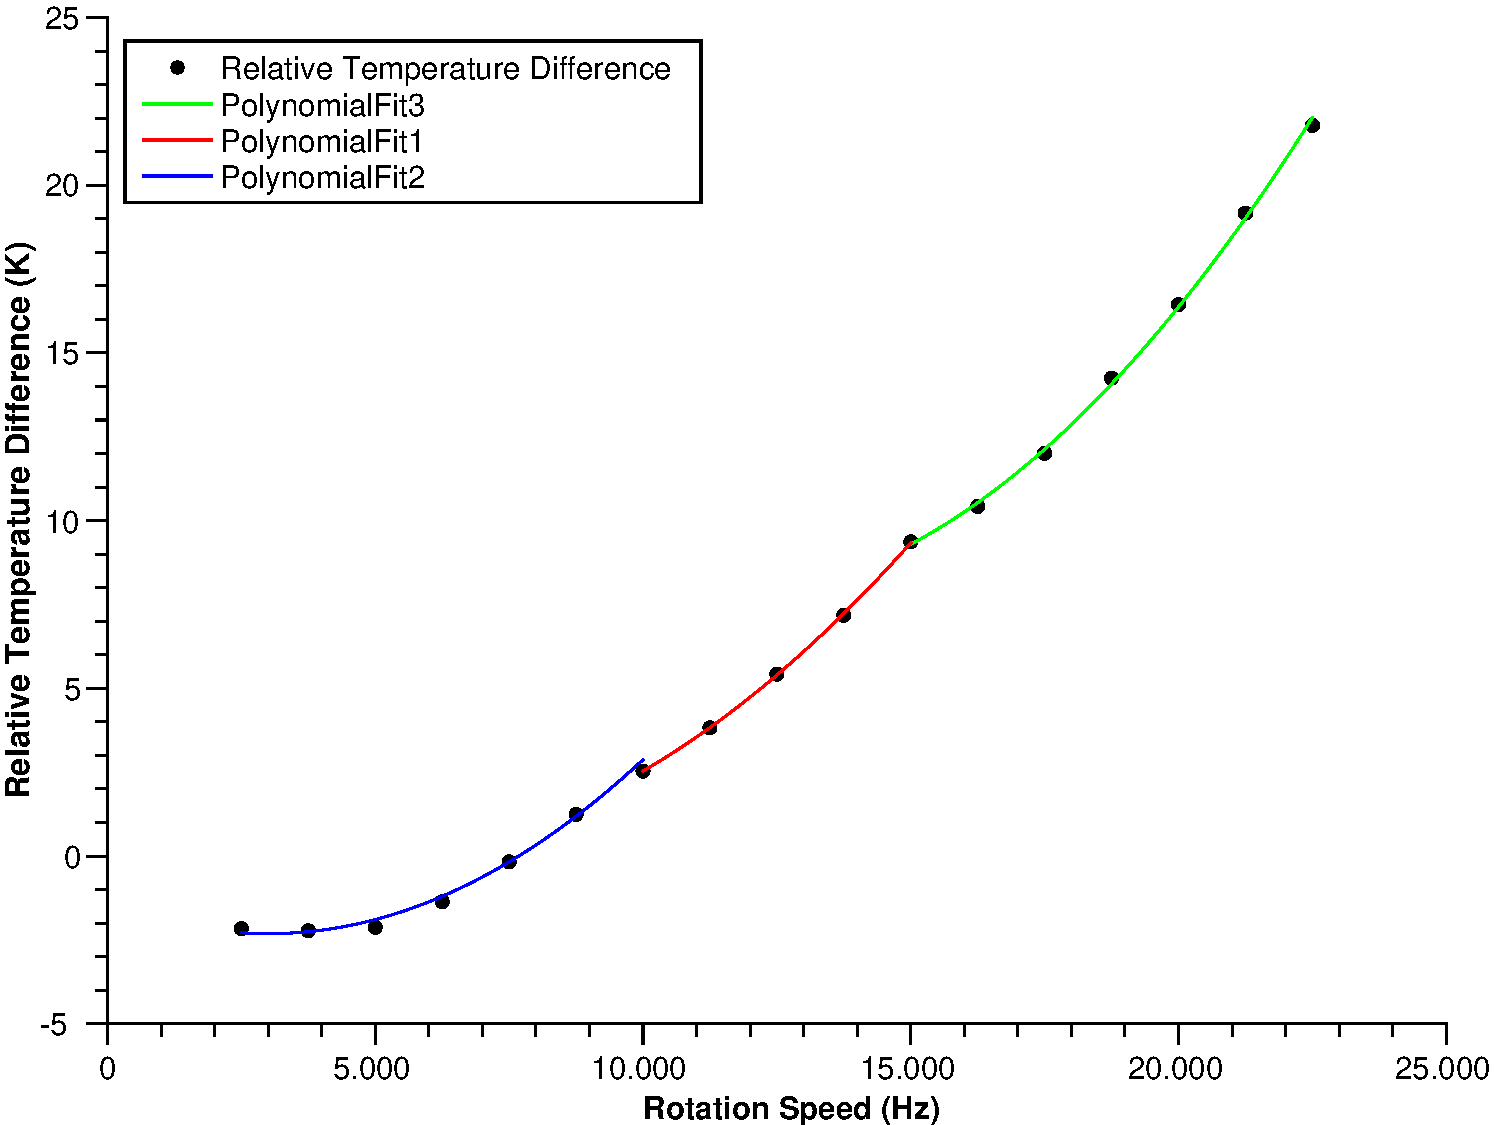
\includegraphics[width=0.7\textwidth]{207Pb/207Pb_250K.pdf}
    \caption{Relative temperature difference as a function of the MAS rotation speed at 250 K}
    \label{fig:207Pb_250K}
\end{figure}
\FloatBarrier

Note that there are three colour-coded regions, to which were individually fitted a parabola. If the fit is done on the whole range, the fit sometimes deviates of up to 3 K from the data point, which is a significant error.

The equations for the fits are the following;
\[
\begin{cases}
    \left. \Delta \theta (\omega) \right|_{\omega \in [2500,10000]} = (1,062156 \cdot 10^{-7}) \omega^2 -(6,401068 \cdot 10^{-4}) \omega - 1,348877 \\ 
    \left. \Delta \theta (\omega) \right|_{\omega \in [10000,15000]} = (8,633959 \cdot 10^{-8}) \omega^2 -(7,981154 \cdot 10^{-4}) \omega + 1,880482 \\ 
    \left. \Delta \theta (\omega) \right|_{\omega \in [15000,22500]} = (1,125679 \cdot 10^{-7}) \omega^2 -(2,524867 \cdot 10^{-3}) \omega + 21,83856 \\ 
\end{cases}
\]  
This wave-like pattern was observed for other experimental conditions as well. It is mysterious however as to why the data doesn't seem to be producing a "smooth" parabola. One hypothesis is that it is linked to the aerodynamics inside the drive and bearing, which change with rotation speed and thus the drag induced isn't purely a parabola either. The airflow inside the capsule containing the sample is quite complicated, as there is an influx of coolant air from the bottom coming in contact with room temperature drive and bearing air flux.

\section{Programming}

Most of the acquisitions done are automated via AU programs. They are using a mix of C++ and Bruker coded functions to interact directly with the spectroscope hardware. There are many of programs that come shipped with the software, however these were not fit for our needs. There was no program to realize acquisitions while incrementing both rotation speed and temperature at the same time. So with a lot of documentation and experimentation to go through, we write our own!

The AU-MULTI-VT-MAS script will make acquisitions according to a list containing pairs of parameters: temperature and rotation speed. The AU-MULTI-VT-STATIC will perform acquisitions while no rotation is happening, however still performs a spinning sequence in order to remove the dipolar coupling effects.

In both scripts, the first part is all about opening the file with the parameters we want, reading and storing them in variables we can use later on. Along the way we need to check for some errors such as file path errors or inexistant and empty files, so a few failsafes are implemented. The second part is then doing the acquisition according to the lists.

With these scripts on hand, we can write down a list and let the computer make the acquisitions by itself, which is particularly handy when conducting lengthy experiments.

\subsection{AU-MULTI-VT-MAS}

\begin{minted}[breaklines=true,breaksymbolleft=,breakindentnchars=2]{c}
/*
  Description:
  This AU programm allows variable temperature and variable speed acquisitions.
  The parameters for the aquisitions need to be passed in in a .txt file, stored in the vt list directory.
  Example of a parameter list: temperature (K) [whitespace] rotation speed (Hz)
    280 2000
    275 10000
    275 15000
  If datasets do not yet exist, the current dataset and its parameters are copied. 
  If the data sets already exist, then the experiments are executed as they are.
  Temperature and rotation speed are set according to the values in the parameter list. You will be asked for the temperature equilibration time. The AU program will wait at as long as defined by this time for the temperature to settle.

  Author: Louis-Hendrik Barboutie
  Email: louis.barboutie@gmail.com

  Modifications:
  - 12/09/2022  changed parameter list format
  - 09/09/2022  created
*/

AUERR = au_multi_vt_mas(curdat);
QUITMSG("--- AU program au_multi_vt_mas finished ---")

#include <inc/exptUtil>

int au_multi_vt_mas(const char* curdat){
  int i;
  int masr_list[128], t_spin, t_before, t_after, experiments_counter, t_equi;
  float temp_list[128];
  char parameter_list_name[PATH_MAX], line[PATH_MAX], parameter_list_path[PATH_MAX];
  FILE *fptr_parameter;
    
  /* input of the temperature and masr lists */
  (void) strcpy (parameter_list_name, "parameterList");
  GETSTRING("enter name of parameter list:", parameter_list_name)
  
  /* get the file path */
  if (getParfileDirForRead(parameter_list_name, VT_DIRS, parameter_list_path) < 0){
    Proc_err(DEF_ERR_OPT, "VT list file %s: %s\n"
		"Please use 'edlist vt' to check for valid files.",
		parameter_list_name, parameter_list_path);
    ABORT
  }

  /* open the files and check for null */
  if ( (fptr_parameter = fopen (parameter_list_path,"r")) == NULL ){
  	Proc_err(DEF_ERR_OPT, "Could not open VT list file\n%s\n"
	  "Please use 'edlist vt' to check for valid files.",
	  parameter_list_path);
   	ABORT
  }	
  	
  /* store temperature and rotation speed settings in a list */
  experiments_counter = 0;
  while (fgets (line, sizeof(line), fptr_parameter) != NULL){
	if (sscanf(line, "%f %i", &temp_list[experiments_counter],
	&masr_list[experiments_counter]) != 2){ break; }
	experiments_counter ++;
  }
        		
  fclose( fptr_parameter );
    
  GETINT("enter thermal equilibration time (sec):", t_equi)
    
  /* test aquisition sequence */
  i = 0;
  TIMES(experiments_counter)
    SETCURDATA
    STOREPAR("TE",temp_list[i]) // set the temperature parameter
    STOREPAR("MASR",masr_list[i]) // set the rotation speed parameter
    STOREPAR("L 31",masr_list[i]) // set the rotation speed parameter
    TESET // set the target temperature
    MASR // set the target rotation speed
    MASG(5) //start the rotation
    TEREADY(t_equi,0.1) // start the temperature change and wait t_equi after stabilization
    ZG_OVERWRITE // do the acquisition
    IEXPNO // increment the experiment
    i++; 
  END
  MASH // halt the rotation
	
  return 0;
}
\end{minted}

\subsection{AU-MULTI-VT-STATIC}

\begin{minted}[breaklines=true,breaksymbolleft=,breakindentnchars=2]{c}
/*
  Description:
  This AU program allows the aquisition of multiple spectra with varying temperature for a static sample, and improves it with a spinning sequence.
  Experiments are created as necessary, but a list containing the temperatures one wants to run the experiment at needs to be written beforehand.
  The sample is given some time (user decided) to equilibrate its temperature before spinning. The spinning is used to obtain a good tensor-shaped peak.
  -------------------------------------------------------------------------
  Author: Louis-Hendrik Barboutie
  Email: louis.barboutie@gmail.com
  -------------------------------------------------------------------------
  Modifications:
  - 12/09/2022  created
*/

AUERR = au_multi_vt_static(curdat);
QUITMSG("---AU program au_multi_vt_static finished ---")

int au_multi_vt_static(const char* curdat){
  FILE *fptr_temperature_list;
  float temperature_list[128];
  int experiments_counter, v_spin, t_spin, i, t_equi;
  char line[PATH_MAX], temperature_list_name[PATH_MAX], temperature_list_path[PATH_MAX];

  /* input of the temperature list */
  (void) strcpy (temperature_list_name, "temperatureList");
  GETSTRING("enter name of temperature list:", temperature_list_name)
		
  /* get the file path */
  if (getParfileDirForRead(temperature_list_name, VT_DIRS, temperature_list_path) < 0){
    Proc_err(DEF_ERR_OPT, "VT list file %s: %s\n"
	"Please use 'edlist vt' to check for valid files.",
	temperature_list_name, temperature_list_path);
    ABORT
    }

  /* open the files and check for null */
  if ( (fptr_temperature_list = fopen (temperature_list_path,"r")) == NULL ){
    Proc_err(DEF_ERR_OPT, "Could not open VT list file\n%s\n"
	  "Please use 'edlist vt' to check for valid files.",
	  temperature_list_path);
    ABORT
    }	
  	
  /* store temperature and rotation speed settings in a list */
  experiments_counter = 0;
  while (fgets (line, sizeof(line), fptr_temperature_list) != NULL){
    if (sscanf(line, "%f", &temperature_list[experiments_counter]) != 1){
      break; 
      }
    experiments_counter ++;
    }
		
  fclose( fptr_temperature_list );

  v_spin = 3000;
  t_spin = 0;
  t_equi = 10;
  GETINT("enter spin rate (Hz) before aquisition:", v_spin)
  GETINT("enter spin duration (sec):", t_spin)
  GETINT("enter equilibration duration (sec):", t_equi)

  STOREPAR("MASR", v_spin) // the spinning sequence uses the same speed each time
  STOREPAR("L 31", v_spin) // both parameters need to be set
  MASR // pass the masr parameter to the spinning unit

  i = 0;
  TIMES(experiments_counter)
      SETCURDATA 
      STOREPAR("TE", temperature_list[i]) // store the next temperature setting from the list in the parameters
      TESET // set the temperature
      TEREADY(t_equi,0.1) // wait until the temperature has stabilized to 0.1 K and then wait t_equi
      MASG(5) // try 5 times to launch the rotation
      sleep(t_spin); // while spinning, wait for t_spin
      MASH // stop the rotation
      sleep(60); // wait 60 sec 
      ZG_OVERWRITE // acquisition
      IEXPNO // experiment incrementation
      i++; 
  END

  return 0;
}
\end{minted}
\section{Observations}

\subsection{Nitrogen and Helium refillings}

The magnet inside the spectroscope has to be cooled to 4 K to become supraconductive, and loose its internal resistance (else it acts as a fuse and the high currents lead to explosive endings). This is achieved with a helium mantle which is itself isolated from the exterior by a mantle of liquid nitrogen. While great care is taken to avoid losses, the evaporation is inevitable. Therefore the Helium and Nitrogen levels have to be periodically checked. The Helium falls to critical levels in about sixth months, whereas Nitrogen in about a week. 

The coolant levels were adjusted on the 500 Mhz and the 750 Mhz spectroscopes. Helium gets refilled by the manufacturer itself, but the Nitrogen is getting refilled by a lab member. There are special chimneys through which each coolant can be introduced into the tanks. A set of manometers and valves measure the evaporation rate and pressure, and can give information on abnormal behaviour of the system.

The state of the coolant levels is logged before and after the refilling. Using a rubber hose, the liquid Nitrogen is transferred from the container to the spectroscope. Since it can freeze and shatter like glass, protective gloves and a visor should be worn during the procedure. 

\subsection{Spinner handling}

Sample spinners have to be filled and cleaned for each experiment, while taking great care in preserving the structural integrity. Replacing a spinner is very costly, and scales with the diminishing diameter.

I have been introduced to filling the 3,2 mm spinner, which has been used to make the temperature studies. The spinners assembly follows these steps: first the zirconium oxide tube is capped with a polymer cap, then the sample can be filled in with a special funnel. A maximum amount of sample needs to be used in order to maximize the signal, but some space needs to be left to put on the drive cap. This is the final step and is the part which will make the sample spin.

For smaller spinners the procedure is more difficult. The diameter makes it hard to see what you are doing with the naked eye. A microscope is used in each step to verify that every action has been correctly performed. The steps are the same as for the larger spinners, but devices manufactured with precision allow better handling and storing of the spinner. One has to ensure there is no dust particles both on the spinner and inside at all cost. If not handled correctly, one risks to break the spinner.

An issue when cleaning the spinner is the removal of caps. More often than not, this leads to permanent deformation of the caps, and therefore a special device has been engineered by Marine Guilmont. It has proven its effectiveness by boosting the success rate of cap removal from 50\% to almost 90\% with minimal damage.

\subsection{Spectroscope settings}

The probe inside the spectroscope is a complex RLC circuit. Since the signal is measured with a coil, the circuits parameters needs to be tuned to maximize the signal. This is achieved by tuning and matching: the with the help of additional inductors and capacitors, the impedance and resonnance frequency can be modified to match the one of the sample. It is a manual process: with the help of a monitoring device, the two settings are adjusted by hand until the circuit is well tuned and matched. This however requires a good circuit to begin with: tuning and matching are only possible in for a certain range of frequencies, so sometimes the circuit itself needs to be modified by swapping some coils.

\subsection{Probe repairs}

While the probes manufacturer can repair or modify faulty hardware, it is both not cost and time effective. When a problem arises, it is handy to perform the repairs ourselves. 

While working with Prof. Nevzorov $^{15}$NH$_4$Cl samples, there was an issue where the frequency couldn't be matched on the $^1$H and $^{15}$N channels (during the "wobble" process). In this case, it was also an experiment to find what to do in order to be able to tune it again. Using trial and error, we identified a certain coil which could be modified by introducing a small metallic piece inside the spires. This brought us closer to the desired frequency, but not quite. Adding another coil in series had a similar effect but was impractical and less effective. In the end we found the problem: it was a grounding issue. As soon as the circuit got grounded the frequency could be set. So the repairs consisted in connecting an already grounded screw to the acquisition circuit. We had to solder small connections and it then proceeded to work flawlessly. 
The next step however was to replace the coil wrapped around the sample, as it had an overly large radius. The field created by the coil was not intense enough for our needs (we only reached about 30 kHz), and a new coil was need. Using a flat wire, we wrapped it around a screw with the desired smaller diameter, creating a coil. Additionally, we increased the number of spires for an even greater effect. With this coil the field strength reached 50 kHz. When testing it with the sample, we noticed it underwent acoustic ringing; this occurs when the frequency going through the surrounding coil is low enough, that the sample has enough time to move slightly under the influence of the electromotive force produced by the coil. Adding an envelope of teflon strap lowered the freedom of movement of the sample and made the acoustic ringing disappear.

\section{Conclusion}

\end{document}